\section{Organizational Hierarchy}
\para{
Hyteno operates with a straightforward organizational structure that encourages collaboration across teams. The company is led by a CEO who oversees several departments, including:  
}

\begin{itemize}
    \item \textbf{Development Team:} Responsible for building and maintaining the software. It is further divided into Frontend Unit and Backend Unit.
    \item \textbf{Design Team:} Focuses on creating user-friendly interfaces and experiences.
    \item \textbf{Operations Team:} Ensures smooth daily operations and project management.
    \item \textbf{Marketing Team:} Promotes Hyteno’s products and services.
    % \item \textbf{Sales Team:} Engages with potential clients and drives sales.
    % \item \textbf{Customer Support Team:} Provides assistance to clients and resolves issues.
    % \item \textbf{Human Resources (HR) Team:} Manages hiring, training, and employee well-being.
\end{itemize}

\begin{figure}[h]
  \centering
  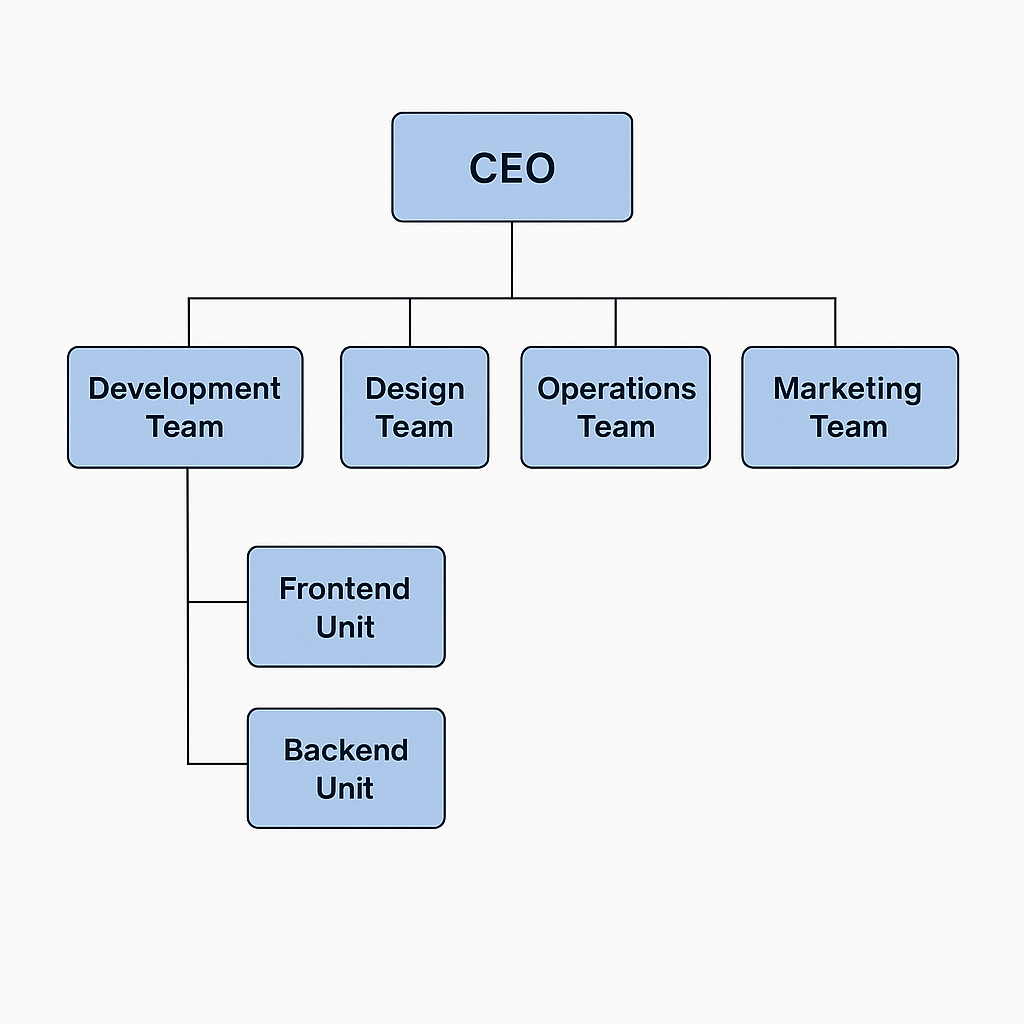
\includegraphics[width=.85\linewidth]{contents/chapters/chapter2/images/Hierarchical-Structure.png}
  \caption{Hyteno Org Chart}\label{fig:example}
\end{figure}

\para{
This structure allows for clear roles and efficient communication, ensuring that projects like Maison Architecture are delivered successfully.
}